\begin{icpcproblem}{G}{Grachten}{Tobias Werth}{2}
Damn! I did not only oversleep (and today is \emph{the} contest day!) but
I also got stuck somewhere in Delft on my way from the hotel to the contest
site. Everywhere around me are grachten, these city-canals that are part of
many cities in the Netherlands. I am in a bit of hurry, because the
NWERC contest starts in a few minutes.

To make matters even worse, some bridges in Delft are closed due to a cycling
race through the city. Thus, I decided to jump over some of the grachten
instead of searching for open bridges.

Everyone knows that computer scientists like me are good at algorithms but
not very good athletes. Besides, I am a bit faint-hearted and don't want to get
wet. So I need your help to calculate the distance I have to
jump over a gracht.

Luckily, I did attend the excursion in Delft city center yesterday, where I
learned that all paving stones in Delft are squares and have the same size.
This way, I can do some measurements on my side of the gracht (my units are
paving stones):

\begin{figure}[h]
	\centering
	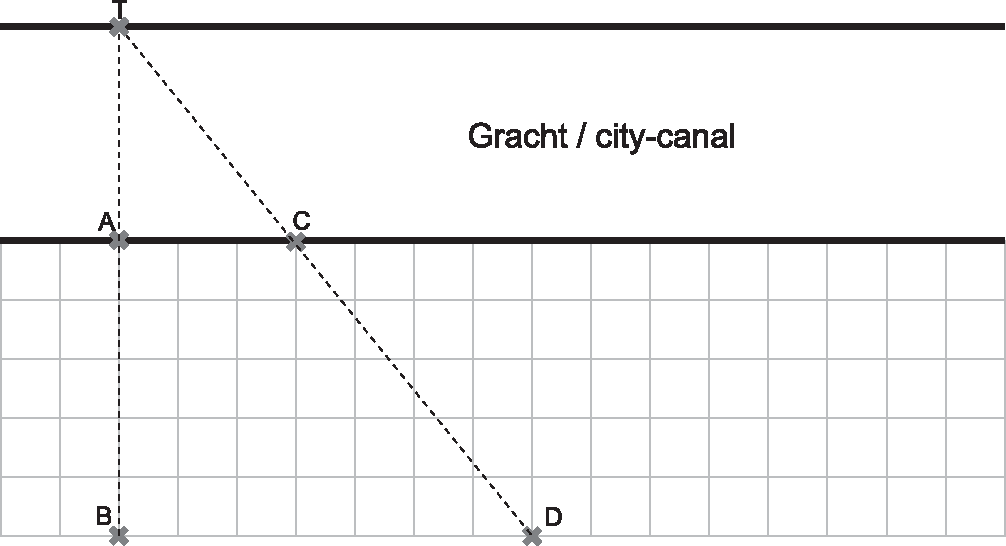
\includegraphics[width=10cm]{gracht}
	\caption{Illustration of first sample input.}
\end{figure}

I walked from point $C$ to point $D$ via points $A$ and $B$ while
counting the paving stones.

Points $A$ and $C$ are always on the edge of the gracht.
Points $B$ and $D$ have the same distance to the gracht.
The target point $T$ is always on the edge of the other side of the canal;
    it is the intersection point of the line through $B$ and $A$, and the line through $D$ and $C$.
The angle between $AT$ and $AC$ is $90$ degrees, and the two edges of the canal are parallel lines.

Please calculate the distance between $A$ and $T$ (necessary jump
distance) for me.

\sectiontitle{Input}

For each test case, the input consists of one line containing three positive integers that
specify the distances between $A$ and $B$, $A$ and $C$, and $B$ and $D$.

You may safely assume that no distance is larger than $1000$ and the distance
between $B$ and $D$ is larger than the distance between $A$ and $C$.

\sectiontitle{Output}

For each test case, print one line of output: the distance between $A$ and $T$ as a {\bf reduced}
fraction (i.e.\ remove all common factors of numerator and denominator).

\sampleio{sample}

\end{icpcproblem}
